\documentclass[journal]{IEEEtran}
\usepackage[a5paper, margin=10mm, onecolumn]{geometry}
\usepackage[cmex10]{amsmath}
\usepackage{amssymb,amsfonts,amsthm}
\usepackage{gvv-book}
\usepackage{gvv}
\usepackage{hyperref}


\begin{document}
\title{8.4.28}
\author{EE25BTECH11025 - Ganachari Vishwambhar}
\maketitle

\textbf{Question}:\\
The diagonal of a rectangular field is 60 metres more than the shorter side. If the longer side is 30 metres more than the shorter side, find the sides of the field.\\
\textbf{Solution: }\\
Let:\\
The shorter side of the rectangle be x\\
The longer side of the rectangle be y\\
Then the diagonal of the rectangle will be $\sqrt{x^2+y^2}$\\
Given:
\begin{align}
    \sqrt{x^2+y^2}=x+60\\
    y^2-120x-3600=0\\
    -x+y=30
\end{align}
Writing equation (3) in conic/quadratic form:
\begin{align}
    \vec{x}^\top A\vec{x}+2\vec{u}^\top\vec{x}+c=0\\
\end{align}
where,
\begin{align}
    A=\myvec{0&0\\0&1}\\
    \vec{u} = \myvec{-60\\0}\\
    c = -3600 
\end{align}
Writing equation(4) in parametric form:
\begin{align}
    \vec{x} = \vec{p} + t\vec{m}
\end{align}
where,
\begin{align}
    \vec{p} = \myvec{0\\30}\\
    \vec{m} = \myvec{1\\1}
\end{align}

Substituting (9) in (4), we get:
\begin{align}
    pt^2+qt+r=0\\
\end{align}
where,
\begin{align}
    p=\vec{m}^\top A\vec{m}\\
    q=2\brak{\vec{p}^\top A\vec{m}+\vec{u}^\top\vec{m}}\\
    r=\vec{p}^\top A\vec{p}+2\vec{u}^\top\vec{p}
\end{align}

By using Sridharacharya's formula,
\begin{align}
    t=\frac{1}{\vec{m}^\top A\vec{m}}\brak{-\vec{m}^\top\brak{A\vec{p}+\vec{u}}\pm\sqrt{\sbrak{\vec{m}^\top\brak{A\vec{p}+\vec{u}}}^2-\brak{\vec{m}^\top A\vec{m}}\brak{\vec{p}^\top A\vec{p}+2\vec{u}^\top\vec{p}}}}
\end{align}

Substituting (17) in (9) we get:
\begin{align}
    \vec{x}= \vec{p}+\frac{1}{\vec{m}^\top A\vec{m}}\brak{-\vec{m}^\top\brak{A\vec{p}+\vec{u}}+\sqrt{\sbrak{\vec{m}^\top\brak{A\vec{p}+\vec{u}}}^2-\brak{\vec{m}^\top A\vec{m}}\brak{\vec{p}^\top A\vec{p}+2\vec{u}^\top\vec{p}}}}\vec{m}\\
    \vec{x}= \vec{p}+\frac{1}{\vec{m}^\top A\vec{m}}\brak{-\vec{m}^\top\brak{A\vec{p}+\vec{u}}-\sqrt{\sbrak{\vec{m}^\top\brak{A\vec{p}+\vec{u}}}^2-\brak{\vec{m}^\top A\vec{m}}\brak{\vec{p}^\top A\vec{p}+2\vec{u}^\top\vec{p}}}}\vec{m}
\end{align}

After substituting values in equation (18) and (19), we get:
\begin{align}
    \vec{p}_1 = \myvec{90\\120}\\
    \vec{p}_2 = \myvec{-30\\0}
\end{align}

Since the side of the rectangle cannot be negative. The correct vector is $\vec{p}_1$.\\ Therefore,
\begin{align}
    x = 90\\
    y = 120
\end{align}

\begin{figure}[h!]
   \centering
   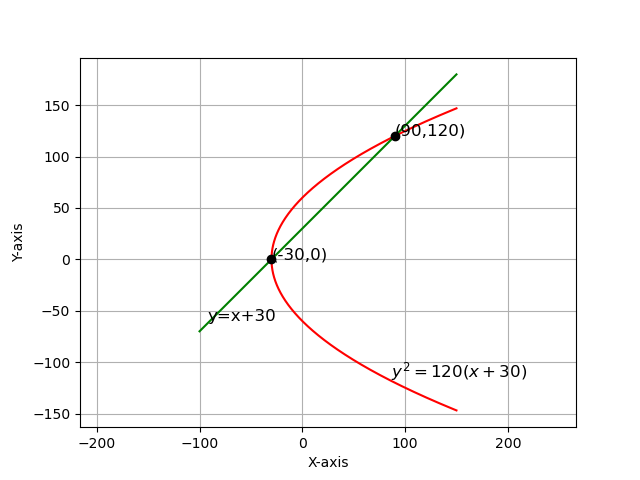
\includegraphics[width=0.7\linewidth]{figs/plot.png}
   \caption{Plot of the parabola and the line}
   \label{}
\end{figure}

\end{document}